\documentclass[main.tex]{subfiles}
\begin{filecontents}{procem.bib}
@book{longair2010high,
  title={High energy astrophysics},
  author={Longair, Malcolm S},
  year={2010},
  publisher={Cambridge university press},
keywords={}
}
@book{longair2003theoretical,
  title={Theoretical concepts in physics: an alternative view of theoretical reasoning in physics},
  author={Longair, Malcolm S},
  year={2003},
  publisher={Cambridge University Press},
  keywords={}
}
@article{passon2017planck,
  title={Planck’s radiation law, the light quantum, and the prehistory of indistinguishability in the teaching of quantum mechanics},
  author={Passon, Oliver and Grebe-Ellis, Johannes},
  journal={European Journal of Physics},
  volume={38},
  number={3},
  pages={035404},
  year={2017},
  publisher={IOP Publishing},
  keywords={}
}
\end{filecontents}
\begin{document}
\part{Stefan-Boltzmann law and LTE}
\begin{itemize}
    \item Radiative transfer equation: atomic emission, absorption and scattering.
    \item LTE
     \item Planck law
\end{itemize}
\chapter{BlackBody Radiation}
\section{Potere emissivo}
Energia emessa per unit\'a di angolo solido, per unit\'a di superficie, per unit\'a di tempo fra $\nu,\nu+d\nu$: $e(\nu,T,x)$.
\begin{figure}
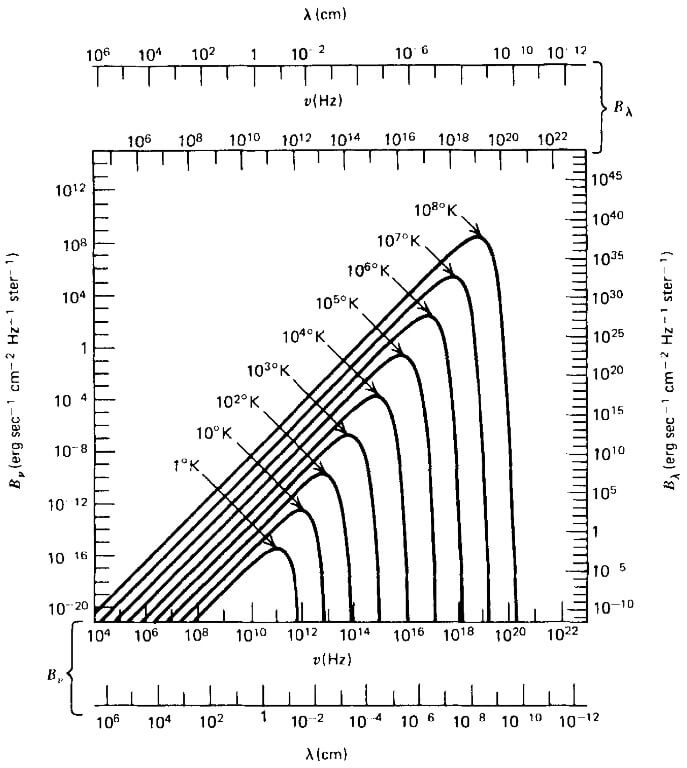
\includegraphics[trim={0cm 0cm 0 0},width=0.9\textwidth]{planckkraus}
%\caption{}
\label{planckkraus}
\end{figure}
\section{Potere Assorbente e corpo nero}
Rapporto tra energia assorbita e energia totale: $a(\nu,T,x)$. Corpo nero ha $a=1$.
\section{Principio di \khhff{}}
\khhff{}(1860) ha dimostrato per via termodinamica che per un corpo in equilibrio termodinamico $\frac{e(\nu,T,x)}{a(\nu,T,x)}$ \'e indipendente da dalla natura del corpo (x): funzione universale $E(T,\nu)$. In una cavit\'a contenente corpi qualsiasi si stabilisce per mezzo di processi irreversibili uno stato stazionario della radiazione che dipende solo da T comune a tutti i corpi: lo stesso stato della radiazione nel vuoto quando le pareti della cavit\'a sono nere e hanno stessa temperatura
\begin{align}
    &\frac{e(\nu,T,x)}{a(\nu,T,x)}=E(\nu,T)\text{P.di\khhff{}}\label{eq:pkhhff}\\
    &e=\int d\,\nu e(\ldots),\ a=\int d\,\nu a(\ldots)
\end{align}
\begin{itemize}
    \item Parte 1.
        \begin{minipage}{\linewidth}
            \centering
            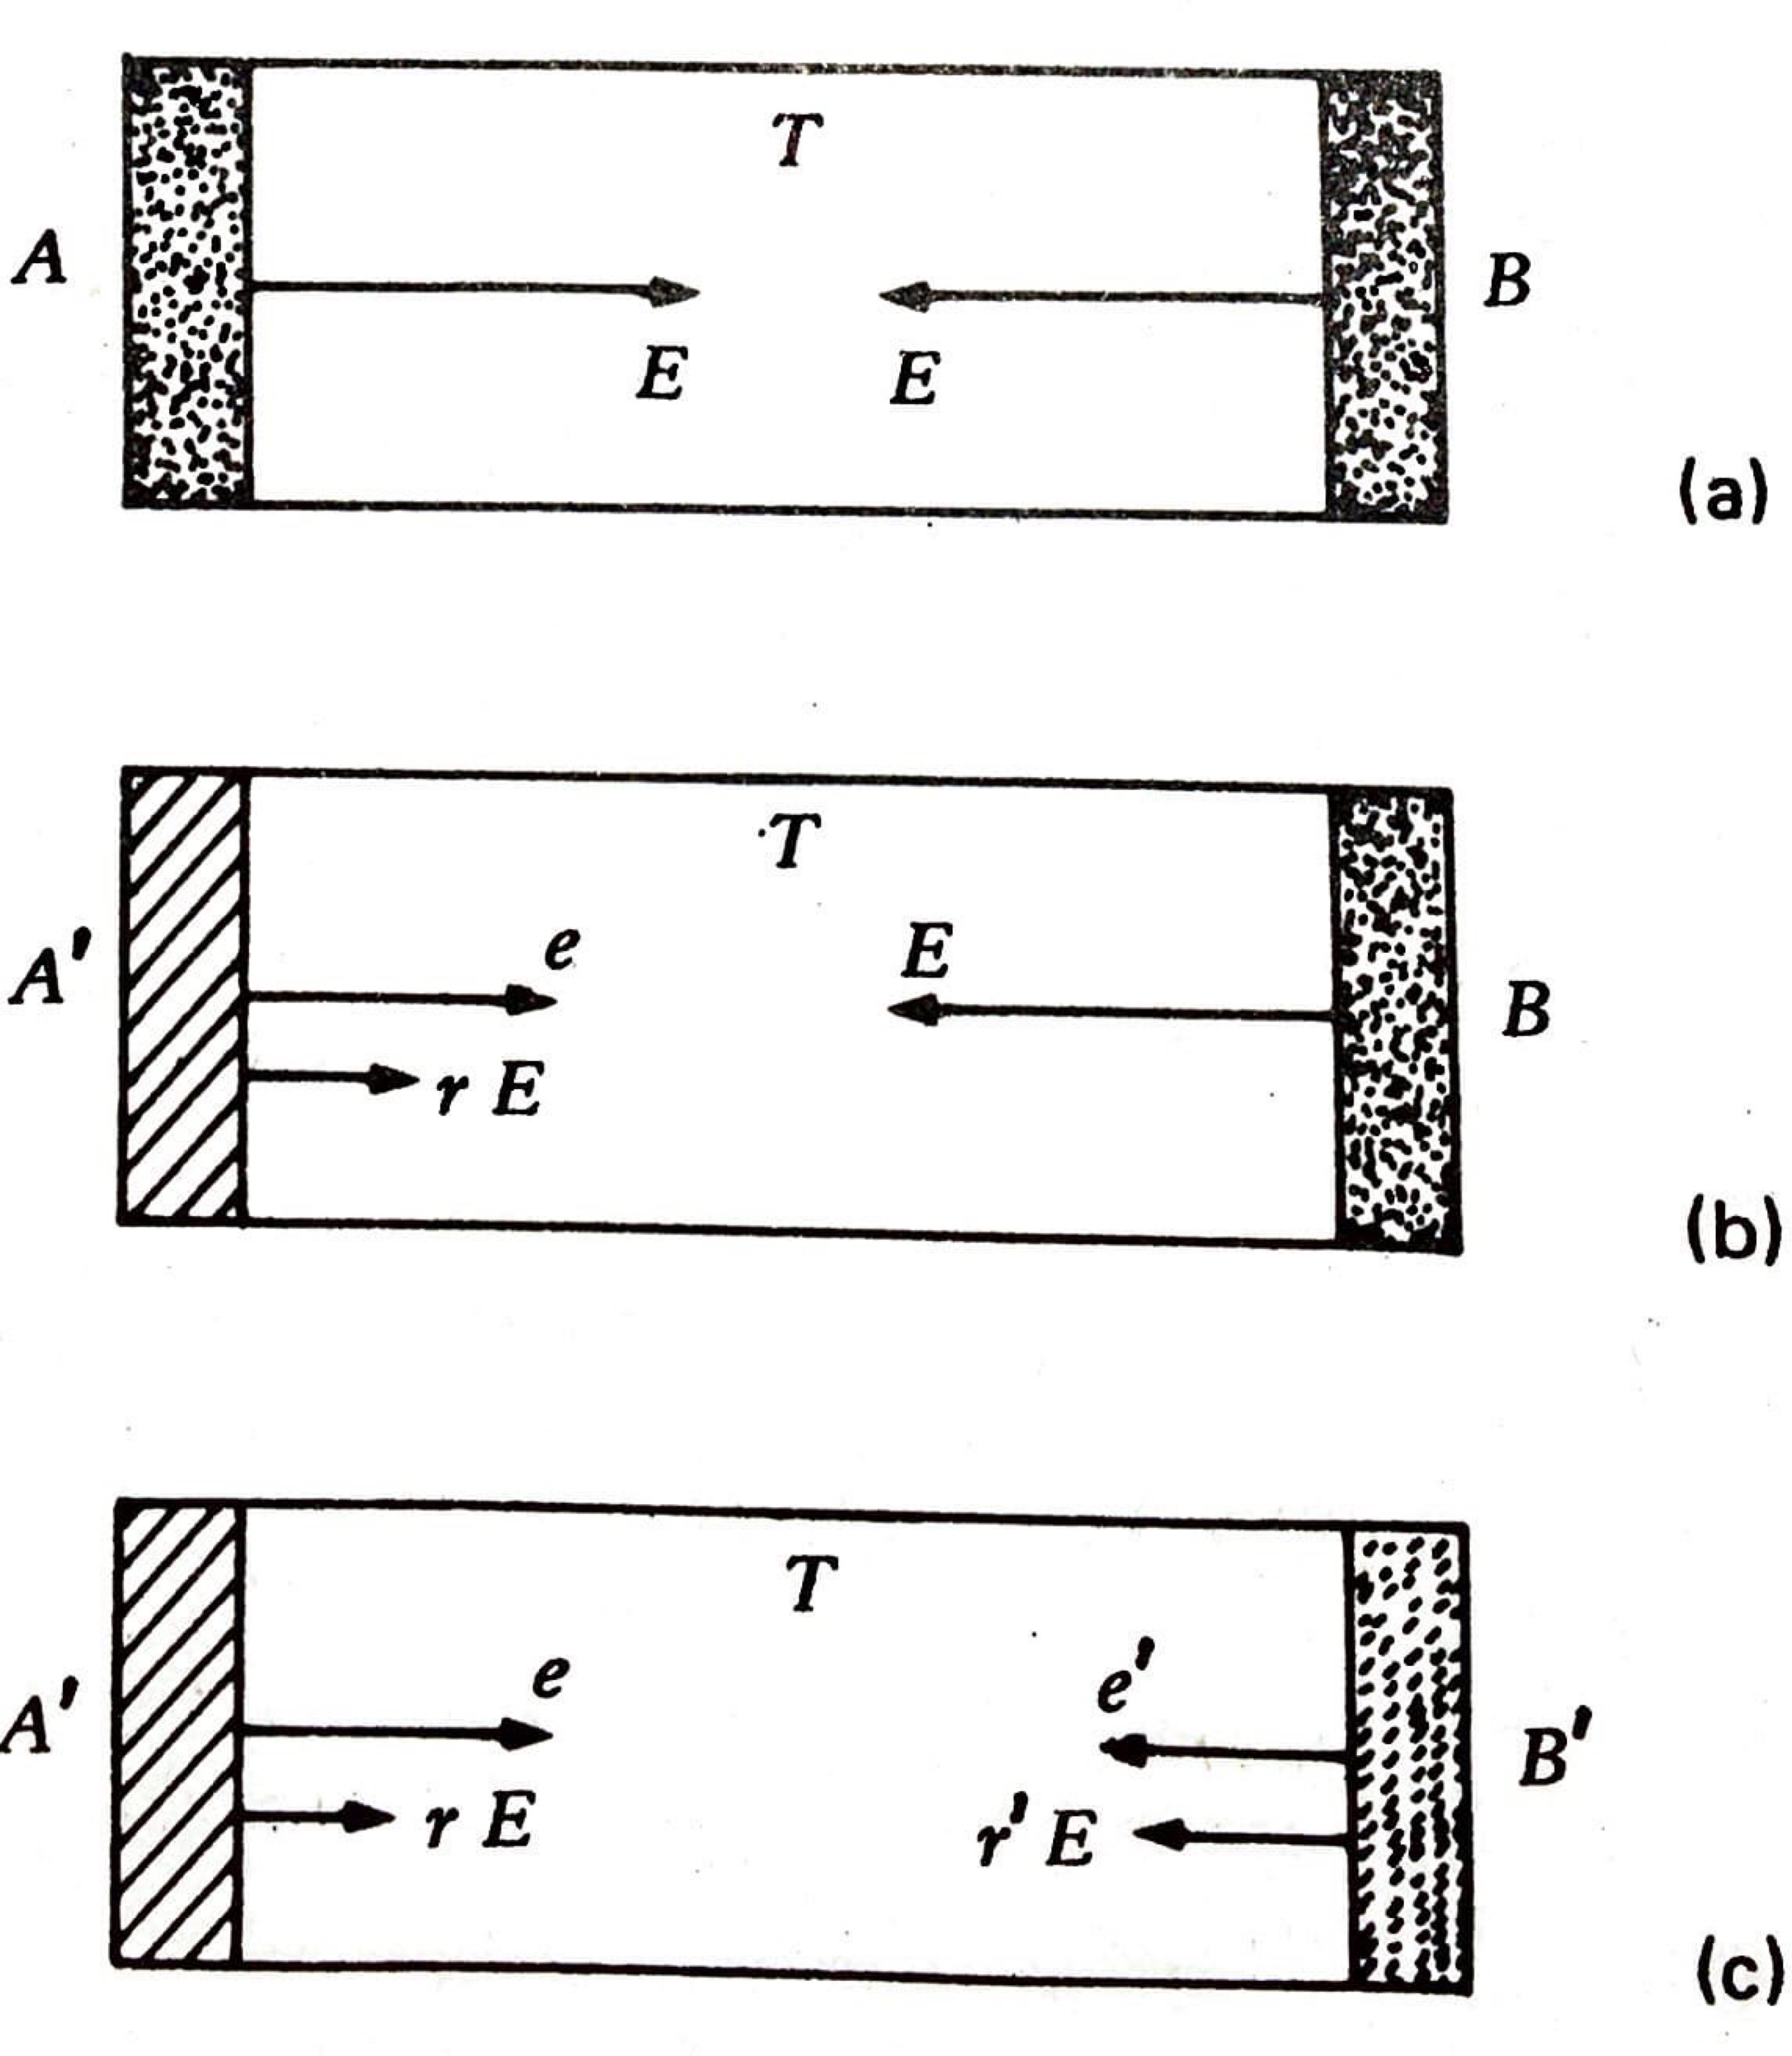
\includegraphics[trim={0cm 0cm 0 0},width=0.9\textwidth]{khhff1}
            %\captionof{khhff1}{Transfer from R1 to R2 whenK1=1}
        \end{minipage}
        Due corpi neri diversi A,B alla stessa temperatura: irraggiamento \'e lo stesso perch\'e se irr. di A fosse maggiore di B la temperatura di B aumenterebbe e diminuirebbe quella di B  - viola secondo principio termodinamica ($\TDy{t}{S}\geq0$: calore ceduto da corpo a temperatura minore negativo assorbito da corpo a temperatura maggiore (+) quindi avremmo diminuzione entropia). In conclusione A e B debìvono irradiare la stessa energia per unit\'a di area.
        Sostituiamo ad A un corpo non perfettamente nero A' dotato di potere emissivo $e$ ed assorbente $a$, E potere emissivo di B di corpo nero: A' emette $e$ \si{\per\square\cm} ed \'e investito da B di cui assorbe $aE$, perch\'e i due corpi si mantengano alla stessa temperatura occorre che $aE=e$ cio\'e $\frac{e}{a}=E$ che non dipende dalla natura del corpo; d'altra parte A' ha potere riflettente r quindi riflette energia $Er$ e all'equilibrio termico l'energia inviata da A' deve eguagliare quella inviata da B $E=(r+a)E=rE+aE=rE+e$, cio\'e A' e B inviano stessa energia.
        Sostituiamo B con B' non nero con potere emissivo $e_1$, assorbente $a_1$, riflettente $r_1$: il corpo $A'$ emette energia $e$ e per conservare T deve ricevere da $B'$ l'energia $Ea$, cio\'e l'energia che $A'$ riceve \si{\per\square\cm} non dipende dalla natura di B.
        Questo vale quando si raggiunge equilibrio termico (equilibrio tra emissione e assorbimento)
    \item Generalizzazione a qualsiasi $\nu$: supponiamo per assurdo che questa relazione non sia valida per tutti i valori di $\nu$. Sia B nero ma A no alla stessa T: tra essi c'\'e lo stesso scambio di energia totale; supponiamo per assurdo:
        \begin{align*}
            e(\nu_1,T,x)d\,\nu>a(\nu_1,T,x)E(\nu_1,T)\\
            e(\nu_2,T,x)d\,\nu<a(\nu_2,T,x)E(\nu_2,T)%\label{}
        \end{align*}
        Supponiamo di dividere il cilindro con una lastra trasparente per l'onda $\nu_1$ e opaca per $\nu_2$ compresa tra due specchi: abbiamo inizialmente due camere distinte nelle quali si stabiliscono radiazioni nere con stessa densit\'a di energia dato che T \'e la stessa ma a sinistra avremo prevalenza di $\nu_1$; togliamo gli specchi: onda $\nu_1$ propaga energia per ristabilire la stessa densit\'a di energia per onda $\nu_1$ ma ci\'o provoca emissione da A e diminuzione di T e aumento di T per B. Assurdo: \ref{eq:pkhhff} \'e valida sempre.
        \begin{minipage}{\linewidth}
            \centering
            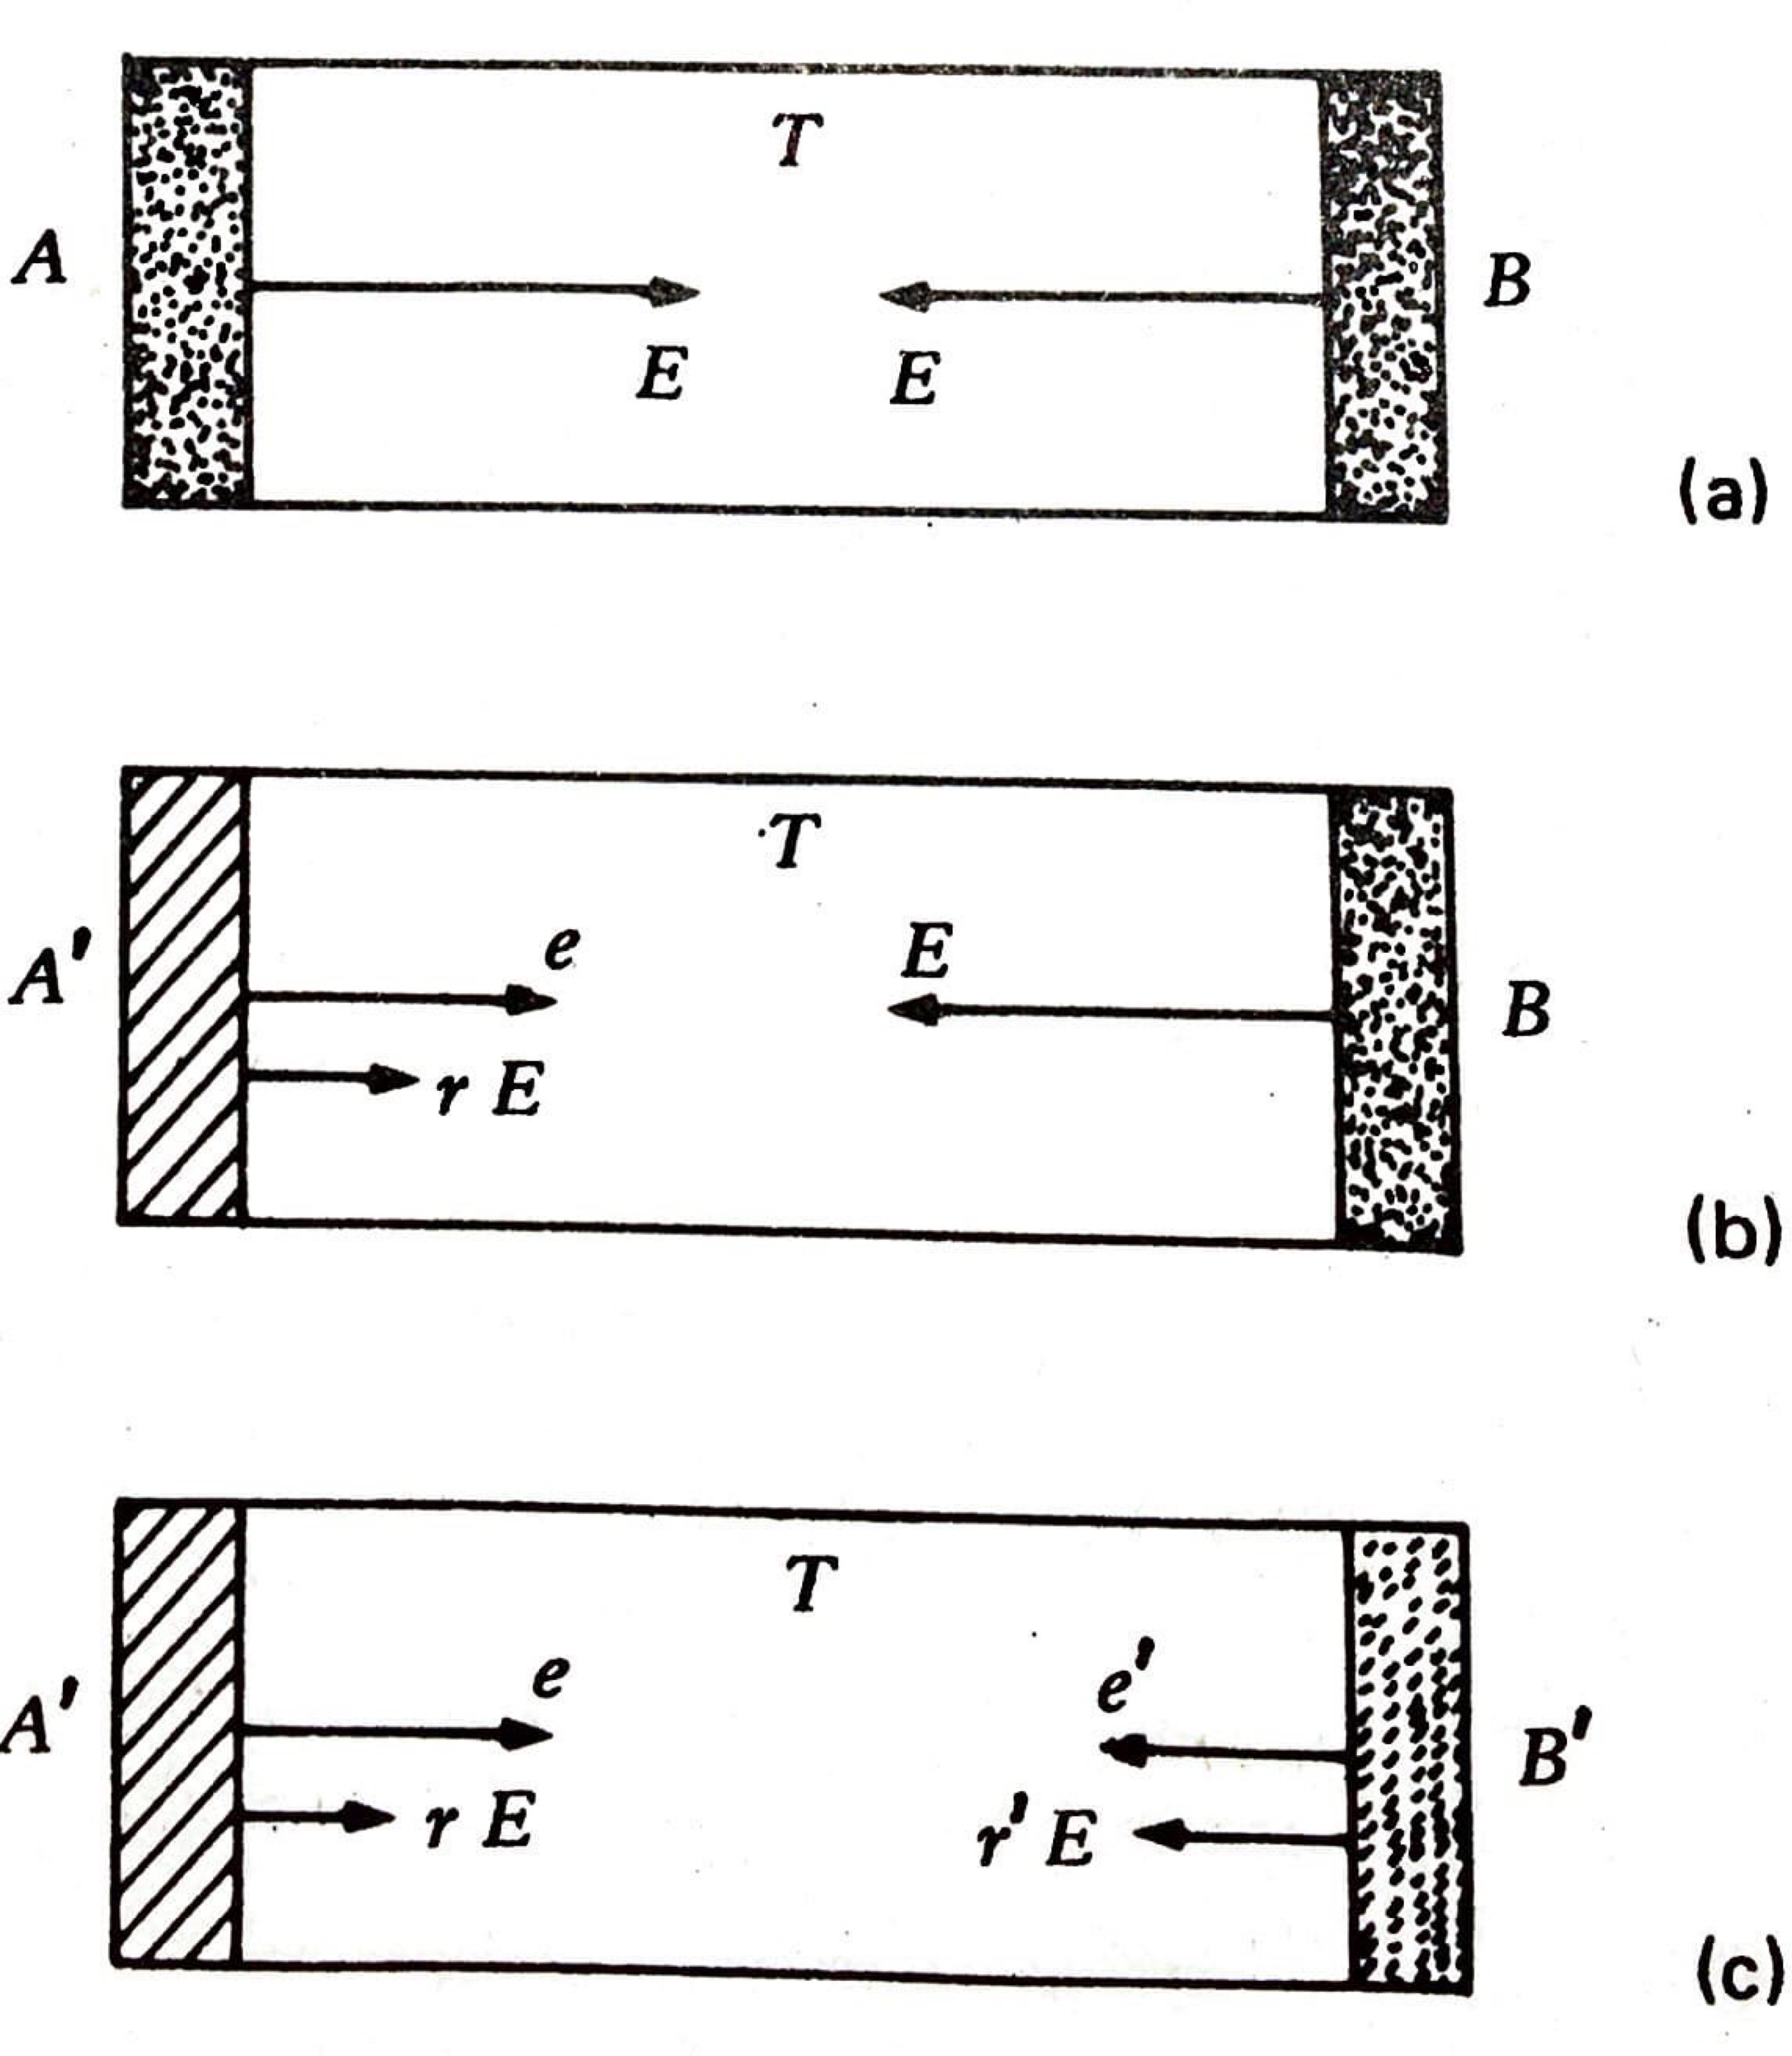
\includegraphics[trim={0cm 0cm 0 0},width=0.9\textwidth]{khhff1}
            %\captionof{khhff1}{Transfer from R1 to R2 whenK1=1}
        \end{minipage}
\end{itemize}
\section{densit\'a energia radiante in una cavit\'a}
Una cavit\'a con pareti assorbenti in euqilibrio termico si ha radiazione nera; determino relazione tra densit\'a di energia della cavit\'a e potere emissivo. Su unit\'a di superficie arriva nell'unit\'a di tempo e per angolo solido $d\,\Omega$ l'energia contenuta entro una distanza percorsa da c in unit\'a di tempo e la stessa energia viene emessa dalla superficie: densit\'a di energia $d(\nu,T)=\frac{2}{c}E(\nu,T)\intd\,\Omega=\frac{4\pi}{c}E(\nu,T)$; analogamnete per corpo non nero $d(\nu,T)=\frac{4\pi}{c}\frac{e(\nu,T,x)}{a(\nu,T,x)}$, ovvero per pareti in equilibrio termico si ottiene relazione precedente.
\section{Pressione di Radiazione: esperimento termodinamico}

\section{Ripeto EM}

\section{Ripeto scattering}


\section{Ripeto statistical physics}

\section{Ripeto QM-Atomo d'idrogeno}

\section{Principio di Kirchhoff}
\khhff{} ha dimostrato per via termodinamica nel 1860 che per un corpo in equilibrio termodinamico
\end{document}
